the face detection step is an essential step before facial expression recognition, as we must first extract the faces from the image before further used for feature extraction (HOG and landmarks) then it's passed to the model.
\newline
we tried multiple face detection approaches that are discussed below.
\subsubsection{lBP classifier face detector}

\paragraph{theory}
Local Binary Pattern (LBP) features have performed very well in various applications, including texture classification and segmentation, image retrieval and surface inspection, for the application of face detection we can make it micro visual patterns in the face.

this classifier divides a given image into blocks, for each block the LBP classifier will consider one window (3X3 window) at a time.\newline

for each window it will compare the center pixel with all other pixels, if a pixel is below the value of centeral pixel its value becomes 0, and 1 otherwise, then the value will be read in clockwise order and form a binary number, which will be the new value of the center pixel as shown in figure \ref{fig:LBP_calculation}.\newline

Then, it converts each block values into a histogram, so now we have gotten one histogram for each block in an image, which are then concatenated together to create a feature vector for the image, this is how LBP features are extracted from the image.

the classifier is then trained on those features with labeled images as faces or non-faces.
\begin{figure}
	\centering
	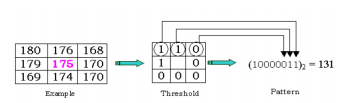
\includegraphics{images/LBP_classifier.png}
	\caption{Example of LBP calculation}
	\label{fig:LBP_calculation}
\end{figure}

\paragraph{performance}
we used the openCV implementation of the LBP classifier, among other methods we tried this was by far \textbf{the the fastest one}, it has an average execution time of 0.812753 seconds, this execution time and performance makes \textbf{it suitable for mobile apps and real time applications} alot, however it's \textbf{very lacking in accuracy and when it comes to small faces mostly wouldn't detect them at all}.

\begin{figure}
	\centering
	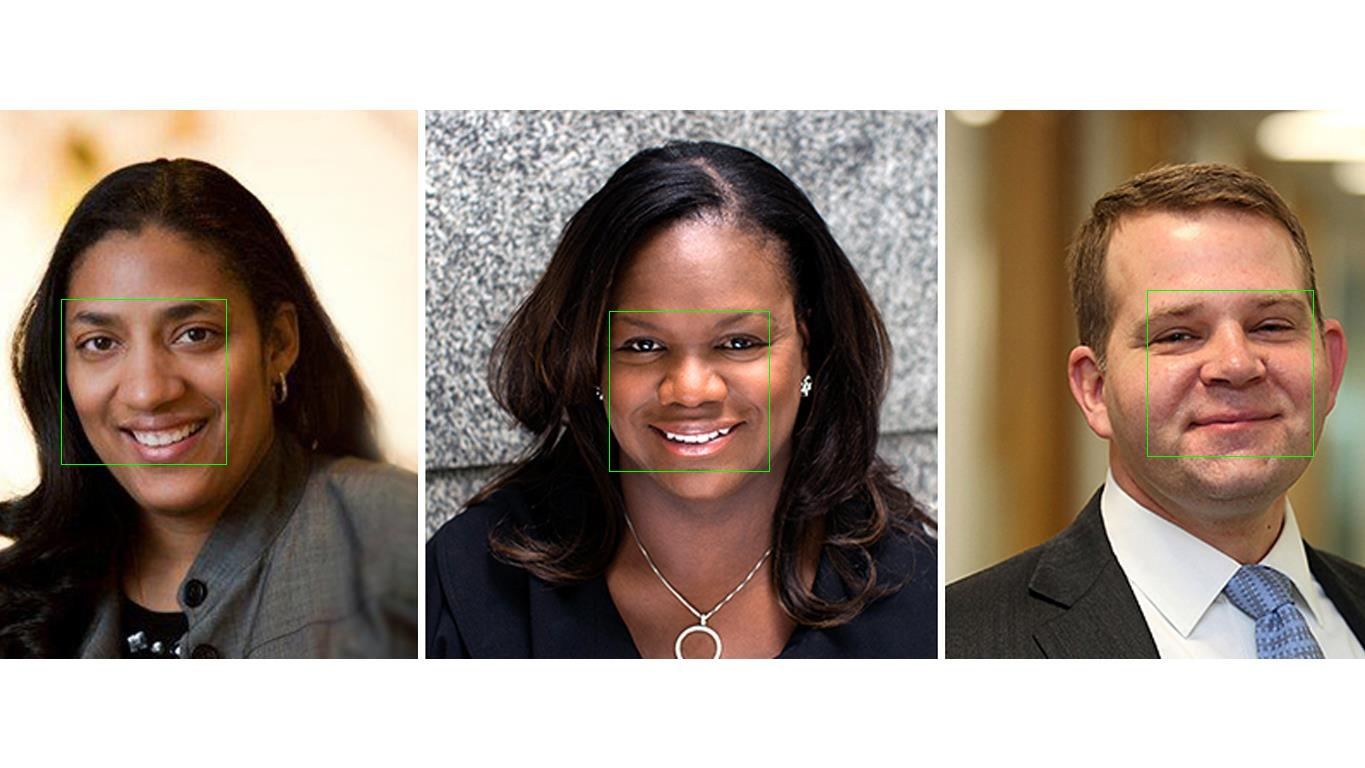
\includegraphics[width=0.75\textwidth]{images/lbp_example.jpg}
	\caption{Example of LBP performance}
	\label{fig:LBP_example}
\end{figure}


\subsubsection{HAAR classifier face detector}

\paragraph{theory}
Object Detection using Haar feature-based cascade classifiers is an effective object detection method proposed by Paul Viola and Michael Jones\cite{haar}, It is a machine learning based approach where a cascade function is trained from a lot of positive and negative images. It is then used to detect objects in other images.

to build the classifier we need a lot of positive images (images of faces) and negative images (images without faces) for training, Then we need to extract features from them, For this, Haar features like those shown in Figure \ref{fig:haar_features} are used, They are just like our convolutional kernel. Each feature is a single value obtained by subtracting sum of pixels under the white rectangle from sum of pixels under the black rectangle.

\begin{figure}
	\centering
	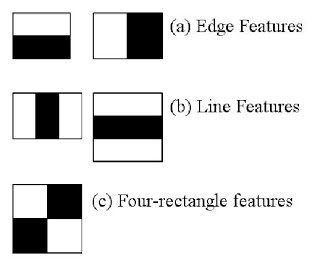
\includegraphics[width=0.5\textwidth]{images/haar_features.jpg}
	\caption{example of haar features}
	\label{fig:haar_features}
\end{figure}

this classifier is a weighed sum of multiple weak classifiers each of which is responsible to detect different features in the face, each of those classifiers has its own threshold value and was trained separately on the given images.
but there are too many features (up to 160000+) which would basically be very time consuming, so we a cascade style classifier, the point of this is that we don't need to test for all features in a window, if the strongest feature isn't there, then we can simply discard it, after few features have been tested we would end up with considerably few windows that can be face candidates, hence greatly increasing the performance, once enough amount of features is found we can accept the candidate window as a face.

\paragraph{performance}
we used the openCV implementation of the HAAR classifier, this classifier is quite close in structure and operation to LBP however \textbf{it has higher accuracy than LBP } as obvious from figure \ref{fig:haar_example} it can even detect most small faces without a problem, however it comes at the cost of execution time which greatly increased to 1.289553 seconds, it's still possible to work with it for real time at soft constraints.
\begin{figure}
	\centering
	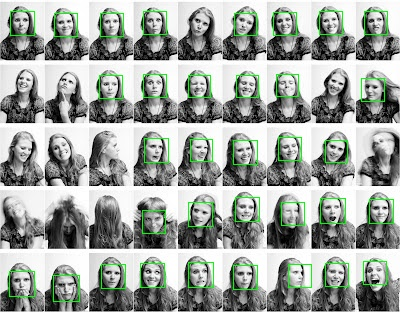
\includegraphics[width=0.75\textwidth]{images/haar_example.jpg}
	\caption{example image displaying the accuracy of HAAR classifier}
	\label{fig:haar_example}
\end{figure}

% big image 2.225201 sec

\subsubsection{Dlib face detector}
\paragraph{theory}
This face detector is made using the Histogram of Oriented Gradients (HOG) feature combined with a linear classifier (linear SVM classifier), an image pyramid, and sliding window detection scheme.
the image pyramid is used to detect faces of different sizes, as it creates multiple images of different resolutions and applies the operation we want to all of them, they are called a pyramid because when the images of different resolutions are stacked with high resolution images at the bottom while low resolution images at he bottom it looks like a pyramid (see Figure \ref{fig:gaussian_pyramid} shows an example of those image pyramid output).
\newline
%to build the pyramid we start by a high resolution image and then reduce its resolution a step by step, each pixel in an image with lower resolution (higher level in the pyramid) would be formed by the contribuion of 5 pixels in the underlying layer using Gaussian weights, so if we start with an $N * M$ image we end up with $N/2 * M/2$ image, so we reduce the image ares to one fourth each time, Figure \ref{fig:gaussian_pyramid} shows an example of those image pyramid output.

the slidig window algorithm is basically a method to pass over the image with a window, at each time only working with one window searching for the object of interest within it, in our case this object is a face.

together those 4 techniques (sliding window algorithm, image pyramid, HOG, SVM) can be used for object detection in general depending on the data set used, of course their parameters would change to match the application of interest.

\begin{figure}
	\centering
	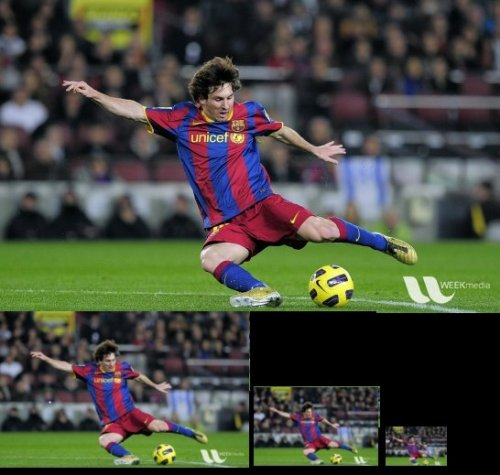
\includegraphics[width=0.75\textwidth]{images/gaussian_pyramid.jpg}
	\caption{Example on Gaussian image pyramid with 4 levels}
	\label{fig:gaussian_pyramid}
\end{figure}

\paragraph{performance}
this is a pre-trained model within the Dlib library, its accuracy can be controlled by an integer input parameter the higher the value the more the accuracy, however this comes at the cost of execution time that would increase as well, after experimentation with it we found value 2 to be good enough, it gives accuracy that is superior to that of HAAR classifier (this can be obvious by comparing Figure \ref{fig:dlib_example} with Figure \ref{fig:haar_example}) with execution time some times even in less than that of HAAR detector, by multiple trials \textbf{we found that its execution time is very dependent on the image size}.

% faces of darbia 0.366657 secs
% example1 3.045794

\begin{figure}
	\centering
	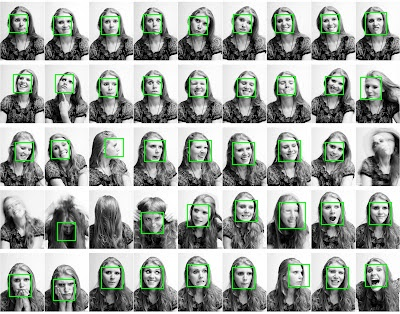
\includegraphics[width=0.75\textwidth]{images/dlib_example.jpg}
	\caption{example image displaying the accuracy of Dlib classifier}
	\label{fig:dlib_example}
\end{figure}

\subsubsection{PCN face detector}
\paragraph{Brief}
it's a \textbf{rotation invariant face detector} made based on Progressive Calibration Networks \cite{PCN}, this approach is one of the most effective approaches to the problem of rotation invariant face detection, it was implemented in c++ using libraries like openCV and Caffe.
\paragraph{theory}
The PCN detector diagram in Figure \ref{fig:PCN_archOverview}, Given an image, all face candidates are obtained according to \textbf{the sliding window and image pyramid principle} ,each candidate window goes through the detector stage by stage, In each stage of PCN, the detector simultaneously rejects most candidates with low face confidences, regresses the bounding boxes of remaining face candidates, and calibrates the RIP orientations of the face candidates. After each stage, non-maximum suppression (NMS) is used to merge those highly overlapped candidates as most existing methods do.
%\begin{figure}
%	\centering
%	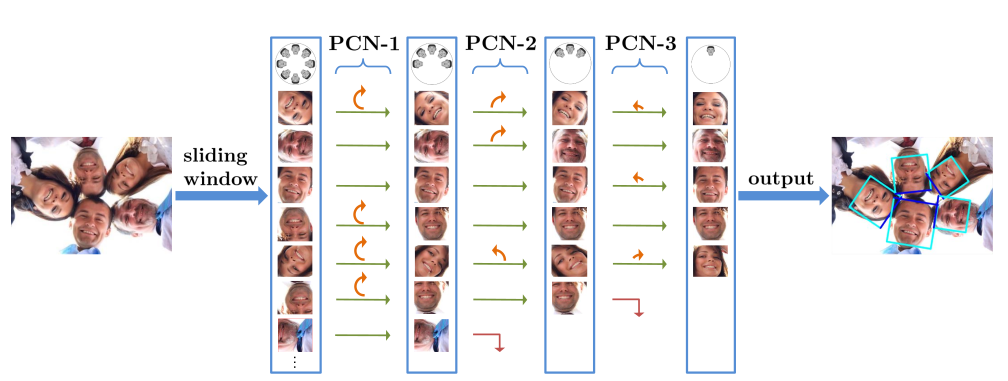
\includegraphics[width=1\textwidth]{images/PCN_archOverview.png}
%	\caption{overview about PCN architecture \cite{PCN}}
%	\label{fig:PCN_archOverview}
%\end{figure}
\paragraph{performance}
this face detection method was by far the best, it was implemented using openCV and Caffe library, its performance in terms of execution time and accuracy surpass the other methods we tried, it even has two main advantages over them as it can't only detect small faces of with high accuracy, it's even rotation invariant and this particular point is what makes it very strong tool.
